%%%%%%%%%%%%%%%%%%%%%%%%%%%%%%%%%%%%%%%%%
% University/School Laboratory Report
% LaTeX Template
% Version 4.0 (March 21, 2022)
%
% This template originates from:
% https://www.LaTeXTemplates.com
%
% Authors:
% Vel (vel@latextemplates.com)
% Linux and Unix Users Group at Virginia Tech Wiki
%
% License:
% CC BY-NC-SA 4.0 (https://creativecommons.org/licenses/by-nc-sa/4.0/)
%
%%%%%%%%%%%%%%%%%%%%%%%%%%%%%%%%%%%%%%%%%

%----------------------------------------------------------------------------------------
%	PACKAGES AND DOCUMENT CONFIGURATIONS
%----------------------------------------------------------------------------------------

\documentclass[
	a4paper, % Paper size, specify a4paper (A4) or letterpaper (US letter)
	10pt, % Default font size, specify 10pt, 11pt or 12pt
]{CSUniSchoolLabReport}


\addbibresource{sample.bib} % Bibliography file (located in the same folder as the template)

%----------------------------------------------------------------------------------------
%	REPORT INFORMATION
%----------------------------------------------------------------------------------------

\title{MA-CSEL \\ Conception systeme Embarqué Linux } % Report title

\author{Kirill \textsc{Goundiaev} \& Tanguy \textsc{Dietrich}} % Author name(s), add additional authors like: '\& James \textsc{Smith}'

\fancyhead[RE,LO]{Kirill Goundiaev \& Tanguy Dietrich}
\fancyhead[CE,CO]{\today}
\fancyhead[LE,RO]{MA-CSEL}

\fancyfoot[RE,LO]{MSE}
\fancyfoot[CE,CO]{\thepage} % this dicard page number dont touch
\fancyfoot[LE,RO]{HES-SO}
\date{\today} % Date of the report


% add image on the left top corner
% Definition of \maketitle
\makeatletter         
\def\@maketitle{
\raggedright
% 
\includegraphics[width = 60mm]{Figures/MSE.png}\\[8ex]

\includegraphics[width = 180mm]{Figures/ImageTitle.png}\\[8ex]
\begin{center}{}
{\Huge \@title }\\[4ex] 
{\Large  \@author}\\[4ex] 
\@date\\[8ex]
% 
\includegraphics[width = 40mm]{Figures/HESSO.png}
\end{center}}
\makeatother

%----------------------------------------------------------------------------------------

\begin{document}

\maketitle % Insert the title, author and date using the information specified above

% add an image
\begin{figure}[H] % Example image
\center{
\includegraphics[width=0.35\linewidth]{EMbeddedLinuxLogo}}
% \caption{Example image.}
\label{fig:speciation}
\end{figure}


%  to make a guard page
\newpage

% generate the summary table
\tableofcontents
\newpage


\section{Objectif}

This is my link: \footnote{\href{http://www.latex-tutorial.com}{http://www.latex-tutorial.com}}.

\section{Programmation Systeme}

\subsection{Systeme de fichier}\label{filesystem}

\subsection{Multiprocessing et Ordonnanceur}\label{multiprocess}
\subsubsection{Exercice 1 Processus et signaux}\label{MPEx1}
Le but de cet exercice etait de mettre en place une communication entre deux processus en utilisant un service linux tel que socketpair.
Le processus enfant devait envoyer des message au processus parent qui devait les afficher. Lorsque le process enfant envoie le message "exit" le programme doit se terminer.
Il etait aussi demander de fixer l'affinité des processus afin que le thread enfant effectue ces taches sur le CPU 1 et le thread parent sur le CPU 0.
Ainsi que d'ignorer les signaux SIGHUP, SIGINT, SIGQUIT, SIGABRT et SIGTERM.\\

Afin d'ignorer les signaux, nous avons utiliser la structure sigaction qui permet de modifier le comportement d'un signal.
Chaque handler de signal a été assigné a SIG\_IGN, ce qui permet d'ignorer le signal.
voici un extrait du code :

\begin{lstlisting}[style=CStyle]
	struct sigaction sa;
	sa.sa_handler = SIG_IGN;
	sigemptyset(&sa.sa_mask);
	sa.sa_flags = 0;
	sigaction(SIGHUP, &sa, NULL);
	sigaction(SIGINT, &sa, NULL);
	sigaction(SIGQUIT, &sa, NULL);
	sigaction(SIGABRT, &sa, NULL);
	sigaction(SIGTERM, &sa, NULL);
\end{lstlisting}
La création du socketpair se fait simplement avec ce bout de code :
\begin{lstlisting}[style=CStyle]
	int fd[2];
    if(socketpair(PF_LOCAL, SOCK_STREAM, 0, fd) < 0) {
        perror("socketpair");
        exit(1);
    }
\end{lstlisting}
Le paramentre PF\_LOCAL permet de créer un socket local, SOCK\_STREAM permet de créer un socket de type TCP. La valeur 0 permet de spécifier le protocole par défaut (ici TCP).

Afin de crée les deux process, nous avons utiliser la fonction fork() qui permet de crée un processus enfant identique au processus parent.
Voici un extrait du programme apres la fonction fork() :
\begin{lstlisting}[style=CStyle]
	pid = fork();
    if (pid == 0) { // child 
        close(fd[PARENTSOCKET]); 
        // set thread affinity
        if(setAffinity(1) == -1) { perror("sched_setaffinity");}
        child(fd[CHILDSOCKET]);
        close(fd[CHILDSOCKET]);
        exit(0);
    }
    else { // parent 
        close(fd[CHILDSOCKET]);
        // set thread affinity
        if(setAffinity(0) == -1) { perror("sched_setaffinity");}
        parent(fd[PARENTSOCKET]);
        close(fd[PARENTSOCKET]);
    }
    // must wait for child to exit
    // waitpid(pid, NULL, 0);
    wait(NULL);
\end{lstlisting}
La valeur de pid retourner par la fonction fork() permet de savoir si le processus est le parent ou l'enfant.
Ensuite il faut assigner l'affinité des processus, pour cela nous avons utiliser la fonction sched\_setaffinity() qui est appelé dans la fonction setAffinity() que nous avons créer.
Pour terminer il ne reste qu'as lancer la fonction correspondante au processus (enfant, ou parent).
Et ne pas oublier d'effectuer un wait pour attendre que le processus enfant se termine. Pour eviter les zombies.
La fonction setAffinity que nous avons créer utilise sched\_setaffinity, voici le code : \\
\begin{lstlisting}[style=CStyle]
	int setAffinity(int core) {
		// set thread affinity
		cpu_set_t cpuset;
		CPU_ZERO(&cpuset);
		// set this process to run on core 0
		CPU_SET(core, &cpuset);
		// here 0 mean use the calling process
		if(sched_setaffinity(0, sizeof(cpuset), &cpuset) == -1) {
	
			return -1;
		}
		return 0;
	}
\end{lstlisting}
La communication entre les deux process est assez simple etant donnée, que nous avons simplement 2 descripteur de fichier, du point de vue de notre programme, c'est comme si nous allions écrire/lire dans un fichier.
Il ne reste plus qu'as lire le descripteur de fichier dans le parent, et d'écrire avec l'enfant.\\
\noindent\begin{minipage}{.50\textwidth}
\begin{lstlisting}[style=CStyle, caption=Processus Enfant]{Name}
void child(int socket) {
	// get the child socket
	int cpt = 0;
	int messageLength;
	bool exitProcess = false;
	while (!exitProcess) {
		messageLength = strlen(messages[cpt])+1;
		write(socket,messages[cpt],messageLength);
		if (strcmp(messages[cpt], EXIT_MESSAGE) == 0) {
			exitProcess = true;
		}
		// juste to give the time to the parent to read the message
		// because the parent could read two message at once and not see the exit message
		usleep(1000000); 
		cpt = (cpt + 1) % NUM_MESSAGE;
	}
	printf("Child exit\r\n");
}
\end{lstlisting}
\end{minipage}\hfill
\begin{minipage}{.45\textwidth}
\begin{lstlisting}[style=CStyle, caption=Processus Parent]{Name}
void parent(int socket) {
	// get the parent socket
	char buffer[512];
	bool exitProcess = false;
	while (!exitProcess) {
		if(read(socket, buffer, sizeof(buffer)) <= 0) {
			perror("read");
			exit(1);
		}
		printf("Parent received: %s\r\n", buffer);
		if (strcmp(buffer, EXIT_MESSAGE) == 0) {
			exitProcess = true;
		}
	}
	printf("Parent exit\r\n");
}
\end{lstlisting}
\end{minipage}
Il faut tout de meme faire attention a plusieurs choses, premierement le parent peut recevoir deux message en meme temps avec la fonction read(), il faut donc faire attention a bien lire le message en entier.
Car on pourrait recevoir "message""exit", avec un zero terminal entre les deux. ce qui ferait que le programme ne s'arreterait pas.
Ensuite la taille du buffer pourrait ne pas etre suffisante pour lire le message en entier, ce qui pourrait crée un buffer overflow.\\

% Synthese de ce qui as été appris/exercé
Lors de ce TP, nous avons appris a utiliser les socketpair afin de communiquer entre deux processus.
Nous avons aussi appris a ignorer des signaux, mais il aurait aussi été possible de les rediriger vers une fonction. Dans le but d'effectuer une action.
Grace a ce TP, nous avons appris a gerer un processus (création, affinité, communication, etc...). En utilisant les fonction fork(), sched\_setaffinity(), socketpair(), etc...\\
% \linebreak

Ce labo a été plus compliquer que nous le pension, car nous avons eut de difficulté pour la reception du message "exit". La solution que nous avons choisit est simple mais pourrait poser des problemes.
Il serait mieux de regarder le nombre de bytes recu, et de parser le message recu dans different string, en utilisant les zero terminal.


\subsubsection{Exercice 2 CGroups Limitation memoire}\label{MPEx2}
% Exercice #2: Concevez une petite application permettant de valider la capacité des groupes de contrôle à limiter l’utilisation de la mémoire.
Dans cet exercice, l'objectif etait de montrer que les CGroups permettent de limiter l'utilisation de la memoire d'un processus.
Pour faire cela, nous avons créer un programme qui alloue de la memoire par block de 2MB, et qui rempli cette memoire avec des 0.
voici ce programme : \\
\begin{lstlisting}[style=CStyle, caption=Allocation de memoire]{Name}
	#define NUM_BLOCKS 50
	#define MEGABYTE 1024 * 1024
	#define BLOCK_SIZE (2 * MEGABYTE)
	
	int main(void)
	{
		int i;
		char *ptr[NUM_BLOCKS];
		printf("Allocating memory...\n");
		for (i = 0; i < NUM_BLOCKS; i++)
		{
			getchar();
			printf("Allocating block %d\n", i);
			ptr[i] = malloc(BLOCK_SIZE * sizeof(char));
			if (ptr[i] == NULL){exit(EXIT_FAILURE);}
			memset(ptr[i], 0, BLOCK_SIZE);
		}
		for (i = 0; i < NUM_BLOCKS; i++){free(ptr[i]);}
		return 0;
	}
\end{lstlisting}
Afin de voir ce qu'il ce passait, nous avons ajouter un print a chaque allocation pour voir a quel moment le programme serait stoppé.
Nous avons aussi ajouter un getchar() afin de pouvoir faire alloué un nouveau block de memoire.
\linebreak
avant de lancer ce code, il est necessaire de créer un groupe de controle, et de limiter la memoire de ce groupe. Afin de simplifier l'utilisation de ce programme, nous avons écrit un script qui permet de faire cela.

\begin{lstlisting}[language=bash]{Name}
#!/bin/sh
mount -t tmpfs none /sys/fs/cgroup
mkdir /sys/fs/cgroup/memory
mount -t cgroup -o memory memory /sys/fs/cgroup/memory
mkdir /sys/fs/cgroup/memory/mem
echo $$ > /sys/fs/cgroup/memory/mem/tasks
echo 20M > /sys/fs/cgroup/memory/mem/memory.limit_in_bytes
./ex2
\end{lstlisting}
Ce script monte un systeme de fichier tmpfs, puis monte un groupe de controle sur ce systeme de fichier.
Ensuite il cree un groupe de controle, et limite la memoire de ce groupe a 20MB a tout les processus qui y sont lié.
Enfin il lance le programme qui alloue de la memoire.

\begin{figure}[H]
	\centering
	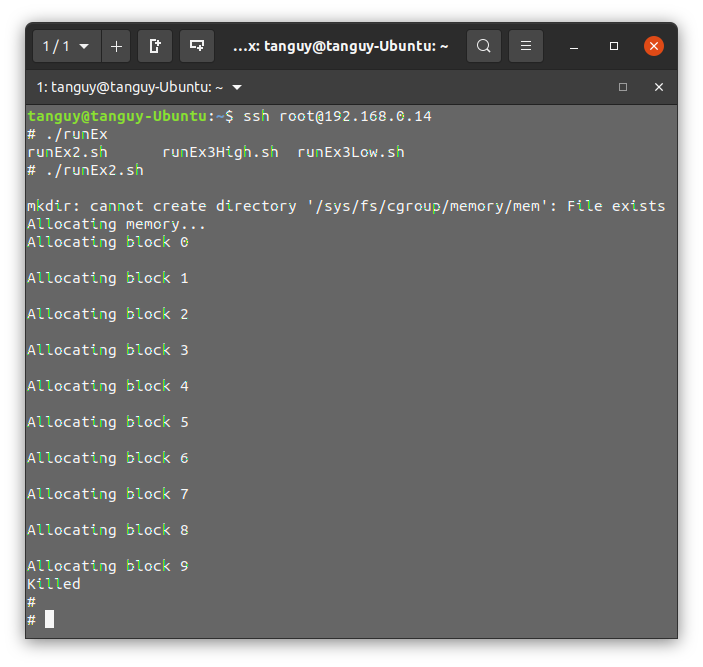
\includegraphics[width=0.4\linewidth]{runEx2}
	\caption{execution de l'exercice 2}
	\label{fig:ex2}
\end{figure}

Comme on peut le voir sur la figure \ref{fig:ex2}, le programme se fait tuer par le kernel lorsque l'on essaie d'allouer le 10eme block de memoire.
Ce qui correspond bien a la limite de 20MB que nous avons fixé.

\begin{enumerate}[label=\textbf{\arabic*}]
	\item \textbf{Quel effet a la commande echo \$\$ > ... sur les cgroups ?}\\
\$\$ en bash est le pid du processus courant. Donc cette commande permet d'écrire le pid du processus courant dans le fichier /sys/fs/cgroup/memory/mem/tasks. Ce qui permet de lier le processus courant au groupe de controle mem.
	
	\item \textbf{Quel est le comportement du sous-système memory lorsque le quota de mémoire est épuisé ? Pourrait-on le modifier ? Si oui, comment ?}\\
Lorsque le quota de memoire est epuisé, le kernel tue le processus qui a essayé d'allouer de la memoire.
Selon cette documentation \footnote{\href{https://access.redhat.com/documentation/en-us/red_hat_enterprise_linux/6/html/resource_management_guide/sec-memory}{https://access.redhat.com/documentation/en-us/red\_hat\_enterprise\_linux/6/html/resource\_management\_guide/sec-memory}}.
Il est possible de legerement modifier le comportement en utilisant le commande :
\begin{lstlisting}[language=bash]{Name}
	echo 1 > /sys/fs/cgroup/memory/mem/memory.oom_control
\end{lstlisting}
Cette commande desactive le "OOM Killer", si un programme atteint ça limite de memoire, il sera mis en pause j'usqu'a ce qu'il y ai de la memoire de disponible.

	\item \textbf{Est-il possible de surveiller/vérifier l’état actuel de la mémoire ? Si oui, comment ?}\\
Afin de surveiller la memoire, il y a plusieur options simple, comme la commande top, htop.
la fonction free permet aussi de voir l'etat de la memoire. Mais elle donne des informations sur la memoire globale, et non sur un processus en particulier.
Il est aussi possible de voir l'etat de la memoire d'un processus en utilisant la commande :
\begin{lstlisting}[language=bash]{Name}
	cat /proc/<PID>/stat | awk '{print $23}'
\end{lstlisting}
\end{enumerate}

% \linebreak

Nous ne conaission pas du tout les CGroups, ce qui a rendu cet exercice tres interessant.
Nous avons réussi a faire effectuer l'exercice, mais a un certain moment la limitation de memoire ne fonctionnait pas.
Il faudrai que l'on regarde plus en detail comment fonctionne les CGroups, et comment les utiliser, la structure et le nombre de fichier present dans le systeme de fichier /sys/fs/cgroup/memory/ est assez impressionant.
Toutefois, il est bon de savoir qu'il est possible de limiter la memoire d'un processus, et de voir comment cela fonctionne.

\subsubsection{Exercice 3 CGroups Controle du CPU}\label{MPEx3}
% Afin de valider la capacité des groupes de contrôle de limiter l’utilisation des CPU, 
% concevez une petite application composée au minimum de 2 processus utilisant le 100% des ressources du processeur.

\section{Conclusion}

%----------------------------------------------------------------------------------------
%	BIBLIOGRAPHY
%----------------------------------------------------------------------------------------

\printbibliography % Output the bibliography

%----------------------------------------------------------------------------------------

\end{document}